\section{Architectural Design and Parameter Formulations}
\label{section:architecture}

This section details the architectural designs, mathematical formulations, and parameter breakdowns for the models investigated in Week 03. All parameter counts are computed directly from tensor layer shapes using standard multiplication without external citations.

\subsection{Pyramid-ResMLP and Pyramid-ResMLP Pure}
\label{subsection:pyramid_resmlp}

Pyramid-ResMLP is a hierarchical MLP-style architecture composed of RepTokenMix blocks and convolutional downsampling stages (Figure~\ref{fig:pyramid_resmlp_arch}). Unlike isotropic columnar MLPs that preserve fixed token sequences across all layers, Pyramid-ResMLP progressively contracts spatial dimensions while expanding channel capacity. We first present the components of the RepTokenMix block and its re-parameterization mechanism in Section~\ref{subsubsection:reptokenmix_components}, describe the overall multi-stage hierarchical architecture in Section~\ref{subsubsection:pyramid_macro}, introduce the PureTokenMix ablation control in Section~\ref{subsubsection:pure_ablation}, and derive the parameter counts in Section~\ref{subsubsection:pyramid_params}.

\begin{figure}[htbp]
\centering
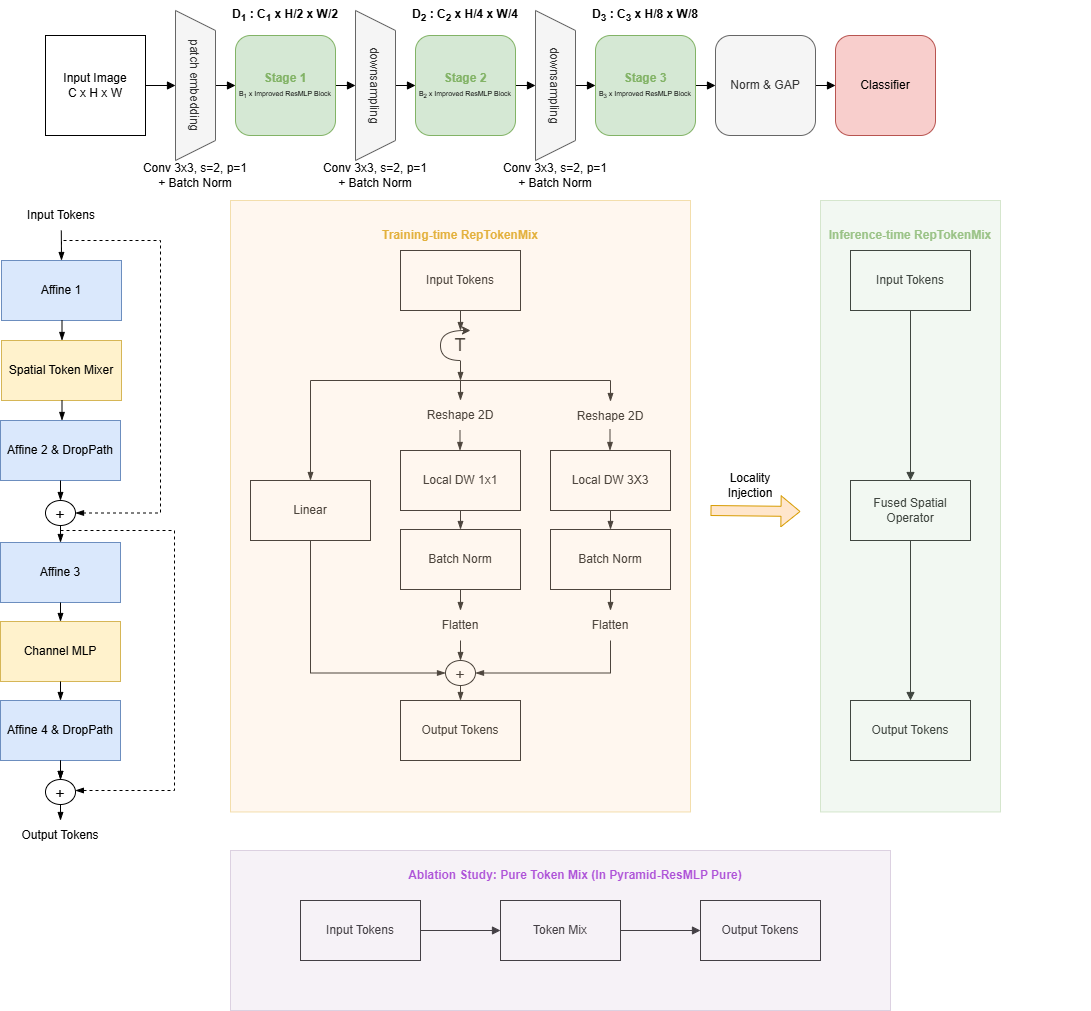
\includegraphics[width=\textwidth]{figures/pyramid_resmlp_and_pure_arch.png}
\caption{Architectural diagrams of Pyramid-ResMLP and Pyramid-ResMLP Pure: 3-stage hierarchical downsampling backbone, training-time re-parameterization in RepTokenMix block, deployment-time locality injection, and the pure linear ablation mixer.}
\label{fig:pyramid_resmlp_arch}
\end{figure}

\subsubsection{Components of RepTokenMix Block}
\label{subsubsection:reptokenmix_components}

A training-time RepTokenMix block is composed of three parallel spatial branches designed to capture multi-scale spatial dependencies: a Global Linear branch, a Local $1*1$ Depthwise Convolution branch, and a Local $3*3$ Depthwise Convolution branch, followed by channel-wise transformation layers (Figure~\ref{fig:pyramid_resmlp_arch}). The outputs of the three spatial components are combined to obtain a comprehensive transformation of the input features before channel mixing.

\textbf{Global linear branch} models long-range, cross-patch spatial dependencies across all $N_i$ token locations simultaneously. Given a sequence of tokens $\mathbf{x} \in \mathbb{R}^{B \times N_i \times C_i}$, the linear branch applies a dense weight matrix $\mathbf{W}_{\text{linear}} \in \mathbb{R}^{N_i \times N_i}$ directly along the transposed token dimension:
\begin{equation}
\mathbf{y}_{\text{linear}} = \mathbf{W}_{\text{linear}} \mathbf{x} + \mathbf{b}_{\text{linear}}.
\end{equation}
While this dense mapping allows any pair of spatial locations to exchange information in a single forward step, it treats all token coordinates as arbitrary permutation-invariant elements, discarding 2D geometric proximity.

\textbf{Local depthwise convolution branches} inject 2D translational equivariance and local spatial inductive bias without cross-channel parameter inflation. In parallel with the global linear branch, the intermediate token sequence is reshaped into a 2D spatial feature map $\mathbf{X} \in \mathbb{R}^{B \times C_i \times H_i \times W_i}$ (where $H_i * W_i = N_i$) and passed through two depthwise convolutional pathways: a $1*1$ depthwise convolution ($\text{Conv2d}(C_i, C_i, k=1, s=1, \text{groups}=C_i) + \text{BN}$) and a $3*3$ depthwise convolution ($\text{Conv2d}(C_i, C_i, k=3, s=1, p=1, \text{groups}=C_i) + \text{BN}$). Because depthwise convolutions apply independent spatial filters within each individual channel, they efficiently capture local edge continuity and adjacent pixel textures. Their outputs are flattened back into $(B, N_i, C_i)$ and combined with the linear projection:
\begin{equation}
\mathbf{y}_{\text{spatial}} = \mathbf{y}_{\text{linear}} + \text{BN}\big(\text{DWConv}_{1\times1}(\mathbf{X})\big) + \text{BN}\big(\text{DWConv}_{3\times3}(\mathbf{X})\big).
\end{equation}

\textbf{Inference-time structural re-parameterization} fuses the parallel convolution and batch normalization branches directly into the weights and biases of a single linear layer upon deployment, achieving zero-overhead locality injection. Because depthwise convolutions and batch normalizations are linear operations with respect to the input tensor, a $3*3$ depthwise convolution acts as a banded, doubly Toeplitz matrix on the flattened token sequence. By passing standard one-hot impulse tensors through the convolution and normalization paths, we extract their exact equivalent matrix transformations $\mathbf{W}_{\text{conv1x1}}, \mathbf{W}_{\text{conv3x3}} \in \mathbb{R}^{N_i \times N_i}$ and bias vectors $\mathbf{b}_{\text{conv1x1}}, \mathbf{b}_{\text{conv3x3}} \in \mathbb{R}^{N_i}$. The final deployed linear mixer is constructed as:
\begin{equation}
\mathbf{W}_{\text{fused}} = \mathbf{W}_{\text{linear}} + \mathbf{W}_{\text{conv1x1}} + \mathbf{W}_{\text{conv3x3}}, \quad \mathbf{b}_{\text{fused}} = \mathbf{b}_{\text{linear}} + \mathbf{b}_{\text{conv1x1}} + \mathbf{b}_{\text{conv3x3}}.
\end{equation}
After fusion, all parallel convolutional branches and batch normalizations are discarded. The deployed network runs as a single dense matrix multiplication $\mathbf{y} = \mathbf{W}_{\text{fused}} \mathbf{x} + \mathbf{b}_{\text{fused}}$, introducing \textbf{zero extra parameters, zero added FLOPs, and zero kernel-launch latency}.

\textbf{Channel MLP and LayerScale} perform cross-channel feature transformations following spatial token mixing. Each block contains two residual sub-layers:
\begin{equation}
\mathbf{x} \leftarrow \mathbf{x} + \text{DropPath}\Big(\boldsymbol{\gamma}_1 \odot \text{TokenMix}\big(\text{Affine}_1(\mathbf{x})\big)\Big),
\end{equation}
\begin{equation}
\mathbf{x} \leftarrow \mathbf{x} + \text{DropPath}\Big(\boldsymbol{\gamma}_2 \odot \text{ChannelMLP}\big(\text{Affine}_2(\mathbf{x})\big)\Big),
\end{equation}
where $\text{Affine}(\mathbf{x}) = \boldsymbol{\alpha} \odot \mathbf{x} + \boldsymbol{\beta}$ is an element-wise affine transformation with learnable scale $\boldsymbol{\alpha}$ and bias $\boldsymbol{\beta}$ that normalizes features without batch-wide communication. The Channel MLP expands channels by a factor of 4: $\text{Linear}(C_i, 4C_i) \rightarrow \text{GELU} \rightarrow \text{Linear}(4C_i, C_i)$. The residual branches are scaled by learnable diagonal LayerScale vectors $\boldsymbol{\gamma}_1, \boldsymbol{\gamma}_2 \in \mathbb{R}^{C_i}$ initialized to $10^{-4}$ to stabilize deep residual learning, and regularized with stochastic depth (DropPath).

\subsubsection{Overall Hierarchical Architecture}
\label{subsubsection:pyramid_macro}

Pyramid-ResMLP arranges RepTokenMix blocks into a progressive 3-stage pyramid backbone (Figure~\ref{fig:pyramid_resmlp_arch}).

\textbf{Overlapping patch embedding stem} replaces standard non-overlapping $4*4$ patch slicing with an overlapping convolution stem:
\begin{equation}
\mathbf{x}_1 = \text{BatchNorm2d}\Big(\text{Conv2d}\big(\mathbf{x}, C_1, k=3, s=2, p=1\big)\Big),
\end{equation}
where $k=3$ is the kernel size, $s=2$ is stride, and $p=1$ is padding. For a $32*32$ CIFAR-100 image, this downsamples the spatial grid to $16*16$ tokens with initial channel capacity $C_1 = 64$. Because neighboring kernels overlap by 1 pixel, boundary artifacts are eliminated while capturing essential low-level edge features. The stem parameter count is:
\begin{equation}
P_{\text{stem}} = \big(C_{\text{in}} * k^2 * C_1 + C_1\big) + 2 * C_1 = \big(3 * 3^2 * 64 + 64\big) + 2 * 64 = 1,792 + 128 = 1,920.
\end{equation}

\textbf{Hierarchical multi-stage backbone} progressively contracts spatial dimensions while doubling channel capacity across three stages ($16*16 \rightarrow 8*8 \rightarrow 4*4$ tokens for $32*32$ input resolution):
\begin{itemize}
    \item \textbf{Stage 1:} Feature map shape $16*16$ ($N_1 = 256$ tokens), channel dimension $C_1 = 64$, depth $B_1 = 2$ blocks.
    \item \textbf{Transition 1 $\rightarrow$ 2:} ConvDownsample module using $\text{Conv2d}(64, 128, k=3, s=2, p=1) + \text{BN}$, halving the spatial resolution to $8*8$ ($N_2 = 64$ tokens) and doubling channels to $C_2 = 128$.
    \item \textbf{Stage 2:} Feature map shape $8*8$ ($N_2 = 64$ tokens), channel dimension $C_2 = 128$, depth $B_2 = 2$ blocks.
    \item \textbf{Transition 2 $\rightarrow$ 3:} ConvDownsample module using $\text{Conv2d}(128, 256, k=3, s=2, p=1) + \text{BN}$, halving the spatial resolution to $4*4$ ($N_3 = 16$ tokens) and doubling channels to $C_3 = 256$.
    \item \textbf{Stage 3:} Feature map shape $4*4$ ($N_3 = 16$ tokens), channel dimension $C_3 = 256$, depth $B_3 = 2$ blocks.
\end{itemize}

\textbf{Convolutional downsample module} employs a strided convolution $\text{Conv2d}(C_{\text{in}}, C_{\text{out}}, k=3, s=2, p=1)$ accompanied by Batch Normalization between stages. This operation performs 2D spatial downsampling with overlapping receptive fields, transforming local patch tokens into semantically rich higher-level visual features. The parameter counts for the two downsamplers are:
\begin{align}
P_{\text{down}, 1\rightarrow2} &= (64 * 3^2 * 128 + 128) + 2 * 128 = 73,856 + 256 = 74,112, \\
P_{\text{down}, 2\rightarrow3} &= (128 * 3^2 * 256 + 256) + 2 * 256 = 295,168 + 512 = 295,680.
\end{align}

\textbf{Classification head} applies Global Average Pooling (GAP) across all spatial tokens of Stage 3, producing a pooled vector $\mathbf{z} \in \mathbb{R}^{C_3}$. An Affine normalization layer and a final linear projection $\text{Linear}(C_3, K)$ output the classification logits for $K=100$ classes:
\begin{equation}
P_{\text{head}} = (2 * C_3) + (C_3 * K + K) = (2 * 256) + (256 * 100 + 100) = 512 + 25,700 = 26,212.
\end{equation}

\subsubsection{PureTokenMix Ablation Architecture (Pyramid-ResMLP Pure)}
\label{subsubsection:pure_ablation}

\textbf{Pure linear token mixer} is constructed as a rigorous ablation control to isolate the exact empirical contribution of the hierarchical multi-stage backbone from that of the structural re-parameterization. Pyramid-ResMLP Pure retains the identical overlapping stem, 3-stage pyramid dimensions, and convolutional downsamplers, but replaces RepTokenMix with PureTokenMix:
\begin{equation}
\mathbf{y} = \mathbf{W}_{\text{spatial}} \mathbf{x} + \mathbf{b}_{\text{spatial}}, \quad \mathbf{W}_{\text{spatial}} \in \mathbb{R}^{N_i \times N_i},
\end{equation}
completely omitting the parallel depthwise convolution and batch normalization branches during training (Figure~\ref{fig:pyramid_resmlp_arch}).

\subsubsection{Mathematical Parameter Breakdown}
\label{subsubsection:pyramid_params}

For CIFAR-100 ($C=[64, 128, 256]$, $B=[2, 2, 2]$):
\begin{itemize}
    \item \textbf{Pyramid-ResMLP (Training):}
      \begin{align}
      P_{\text{train}} &= P_{\text{stem}} + P_{\text{down}} + \sum_{i=1}^{3} B_i * \big(P_{\text{RepToken}, i} + P_{\text{ChannelMLP}, i} + P_{\text{Affine}, i} + P_{\text{LayerScale}, i}\big) + P_{\text{head}} \nonumber \\
      &= 1,920 + 369,792 + 1,540,608 + 26,500 = \mathbf{1,938,820}.
      \end{align}
    \item \textbf{Pyramid-ResMLP (Deploy / Fused):}
      Eliminating the DWConv kernels and BN parameters across all 6 blocks removes:
      \begin{align}
      \Delta P &= 2 * (64*1 + 64*9 + 4*64) + 2 * (128*1 + 128*9 + 4*128) \nonumber \\
      &\quad + 2 * (256*1 + 256*9 + 4*256) = 152,992.
      \end{align}
      Yielding deployable parameters:
      \begin{equation}
      P_{\text{deploy}} = 1,938,820 - 152,992 = \mathbf{1,785,828}.
      \end{equation}
    \item \textbf{Pyramid-ResMLP Pure:}
      Contains no parallel conv branches during training:
      \begin{equation}
      P_{\text{pure}} = \mathbf{1,926,276}.
      \end{equation}
      This is exactly 12,544 parameters fewer than the training-time Pyramid-ResMLP, and 140,448 parameters larger than the deployable Pyramid-ResMLP (due to differences in classification head norm parametrization).
\end{itemize}

\subsection{Shift-ResMLP: Parameter-Free Spatial Communication}
\label{subsection:shift_resmlp}

Shift-ResMLP explores an orthogonal question: \textit{Can spatial communication be achieved with strictly zero learnable parameters?} (Figure~\ref{fig:shift_resmlp_arch}). We first introduce the components of the Shift-ResMLP block in Section~\ref{subsubsection:shift_block}, describe the four-direction spatial shift mechanism in Section~\ref{subsubsection:shift_mechanism}, and derive the parameter counts in Section~\ref{subsubsection:shift_params}.

\begin{figure}[htbp]
\centering
\begin{subfigure}[b]{\textwidth}
    \centering
    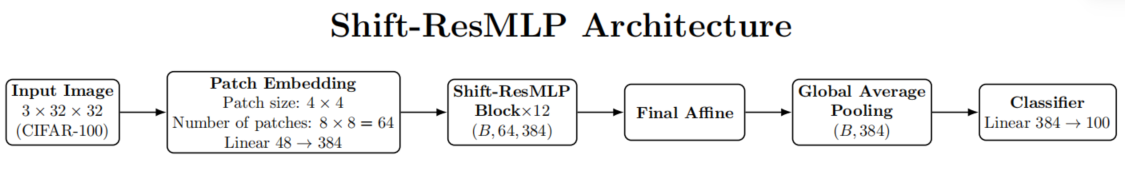
\includegraphics[width=0.98\textwidth]{figures/shift_resmlp_arch_official.png}
    \caption{Macro-architecture of Shift-ResMLP on CIFAR-100.}
    \label{fig:shift_resmlp_macro}
\end{subfigure}
\vspace{0.3em}
\begin{subfigure}[b]{\textwidth}
    \centering
    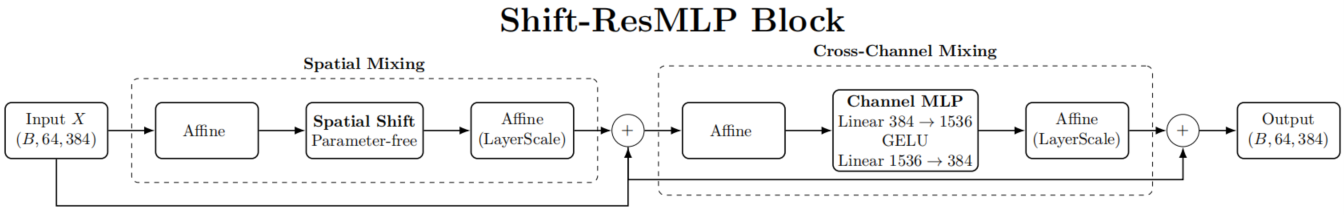
\includegraphics[width=0.98\textwidth]{figures/shift_resmlp_block.png}
    \caption{Shift-ResMLP block structure separating spatial mixing from cross-channel mixing.}
    \label{fig:shift_resmlp_block}
\end{subfigure}
\vspace{0.3em}
\begin{subfigure}[b]{0.63\textwidth}
    \centering
    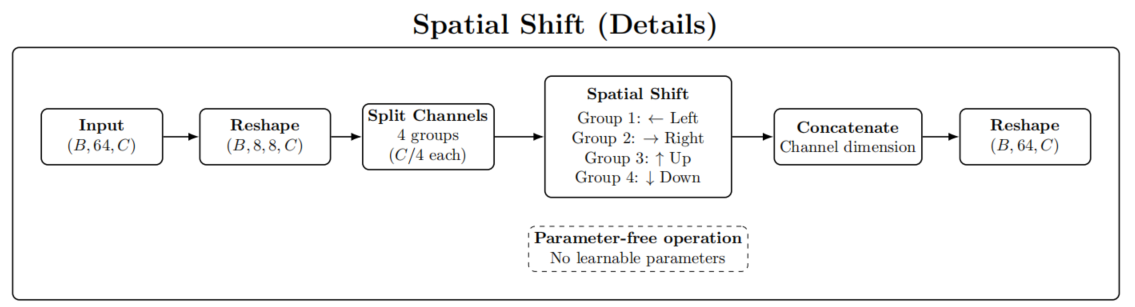
\includegraphics[width=\textwidth]{figures/spatial_shift_details.png}
    \caption{Parameter-free 4-direction coordinate shift mechanism.}
    \label{fig:spatial_shift_details}
\end{subfigure}
\hfill
\begin{subfigure}[b]{0.35\textwidth}
    \centering
    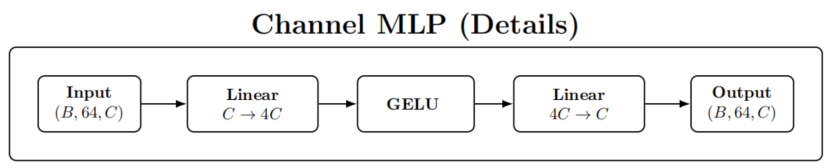
\includegraphics[width=\textwidth]{figures/channel_mlp_details.png}
    \caption{Channel MLP expansion.}
    \label{fig:channel_mlp_details}
\end{subfigure}
\vspace{0.3em}
\caption{Complete architectural design of Shift-ResMLP: macro dataflow, block-level residual paths, parameter-free 4-direction spatial communication, and channel feedforward projection.}
\label{fig:shift_resmlp_arch}
\end{figure}

\subsubsection{Components of Shift-ResMLP Block}
\label{subsubsection:shift_block}

A Shift-ResMLP block consists of two distinct sub-layers: a parameter-free spatial shift sub-layer and a cross-channel MLP sub-layer (Figure~\ref{fig:shift_resmlp_block}).

\textbf{Spatial mixing sub-layer} routes spatial information across tokens without matrix multiplication. Input tokens $\mathbf{x} \in \mathbb{R}^{B \times N \times C}$ are pre-normalized by an Affine layer and fed to the SpatialShift operator. The output is scaled by LayerScale parameter $\boldsymbol{\gamma}_1 \in \mathbb{R}^C$ and added back through a residual connection:
\begin{equation}
\mathbf{x} \leftarrow \mathbf{x} + \boldsymbol{\gamma}_1 \odot \text{SpatialShift}\big(\text{Affine}_1(\mathbf{x})\big).
\end{equation}

\textbf{Cross-channel mixing sub-layer} performs channel-wise feature transformation following spatial communication. Features pass through Affine normalization and a standard two-layer feedforward network: $\text{Linear}(C, 4C) \rightarrow \text{GELU} \rightarrow \text{Linear}(4C, C)$, scaled by LayerScale parameter $\boldsymbol{\gamma}_2$ and added to the residual path (Figure~\ref{fig:shift_resmlp_block}, \ref{fig:channel_mlp_details}):
\begin{equation}
\mathbf{x} \leftarrow \mathbf{x} + \boldsymbol{\gamma}_2 \odot \text{ChannelMLP}\big(\text{Affine}_2(\mathbf{x})\big).
\end{equation}

\subsubsection{Four-Direction Spatial Shift Mechanism}
\label{subsubsection:shift_mechanism}

\textbf{Coordinate feature partitioning} reshapes the 1D token sequence $\mathbf{x} \in \mathbb{R}^{B \times N \times C}$ into a 2D spatial feature map $\mathbf{X} \in \mathbb{R}^{B \times H \times W \times C}$, where $H = W = 32 / 4 = 8$ for patch size $P = 4$ on CIFAR-100. The channel dimension $C$ is partitioned into four equal, non-overlapping subsets of size $c = C / 4$ (Figure~\ref{fig:spatial_shift_details}):
\begin{enumerate}
    \item \textbf{Group 1 (Left Shift):} Channels $[0, c)$ are shifted left by 1 token and zero-padded on the right boundary:
      $\mathbf{X}'_{:, :, :-1, 0:c} = \mathbf{X}_{:, :, 1:, 0:c}$.
    \item \textbf{Group 2 (Right Shift):} Channels $[c, 2c)$ are shifted right by 1 token and zero-padded on the left boundary:
      $\mathbf{X}'_{:, :, 1:, c:2c} = \mathbf{X}_{:, :, :-1, c:2c}$.
    \item \textbf{Group 3 (Up Shift):} Channels $[2c, 3c)$ are shifted up by 1 token and zero-padded on the bottom boundary:
      $\mathbf{X}'_{:, :-1, :, 2c:3c} = \mathbf{X}_{:, 1:, :, 2c:3c}$.
    \item \textbf{Group 4 (Down Shift):} Channels $[3c, 4c)$ are shifted down by 1 token and zero-padded on the top boundary:
      $\mathbf{X}'_{:, 1:, :, 3c:4c} = \mathbf{X}_{:, :-1, :, 3c:4c}$.
\end{enumerate}

\textbf{Receptive field expansion} flattens the concatenated shifted tensor back to $(B, N, C)$. Because each block translates channels by 1 token in four orthogonal directions, stacking $L = 12$ blocks gradually broadens the effective receptive field across the entire $8*8$ grid, enabling global communication through repeated channel MLP mixing.

\subsubsection{Parameter Implications and Baseline Comparison}
\label{subsubsection:shift_params}

The SpatialShift operation contains \textbf{0 learnable parameters}. All model capacity resides in the linear patch embedding ($3 * 4^2 * C + C$) and the channel MLPs ($2 * C * 4C + 5C$ per block). For the experimental setting of $D = 384$ and $L = 12$ blocks:
\begin{equation}
P_{\text{Shift-ResMLP}} = 18,816 + 12 * 1,181,568 + 39,268 = \mathbf{14,264,548}.
\end{equation}
Compared to a standard columnar ResMLP of identical dimensions (ResMLPv2, with 14,314,468 parameters), Shift-ResMLP eliminates exactly $12 * (64 * 64 + 64) = 49,920$ spatial weights while preserving full 2D spatial connectivity.

\subsection{CA-Mixer: Resolution-Agnostic Cellular Automata}
\label{subsection:ca_mixer}

CA-Mixer addresses the resolution-locking bottleneck inherent in vision MLPs (Figure~\ref{fig:ca_mixer_arch}, \ref{fig:ca_scaling}). When image resolution increases from $32*32$ ($N=64$) to $64*64$ ($N=256$), a standard dense matrix $\mathbf{W} \in \mathbb{R}^{64 \times 64}$ fails due to dimensional mismatch. CA-Mixer resolves this by reformulating token mixing as an iterative Neural Cellular Automata (NCA) dynamical system~\cite{mordvintsev2020growing}. We describe its components below.

\begin{figure}[htbp]
\centering
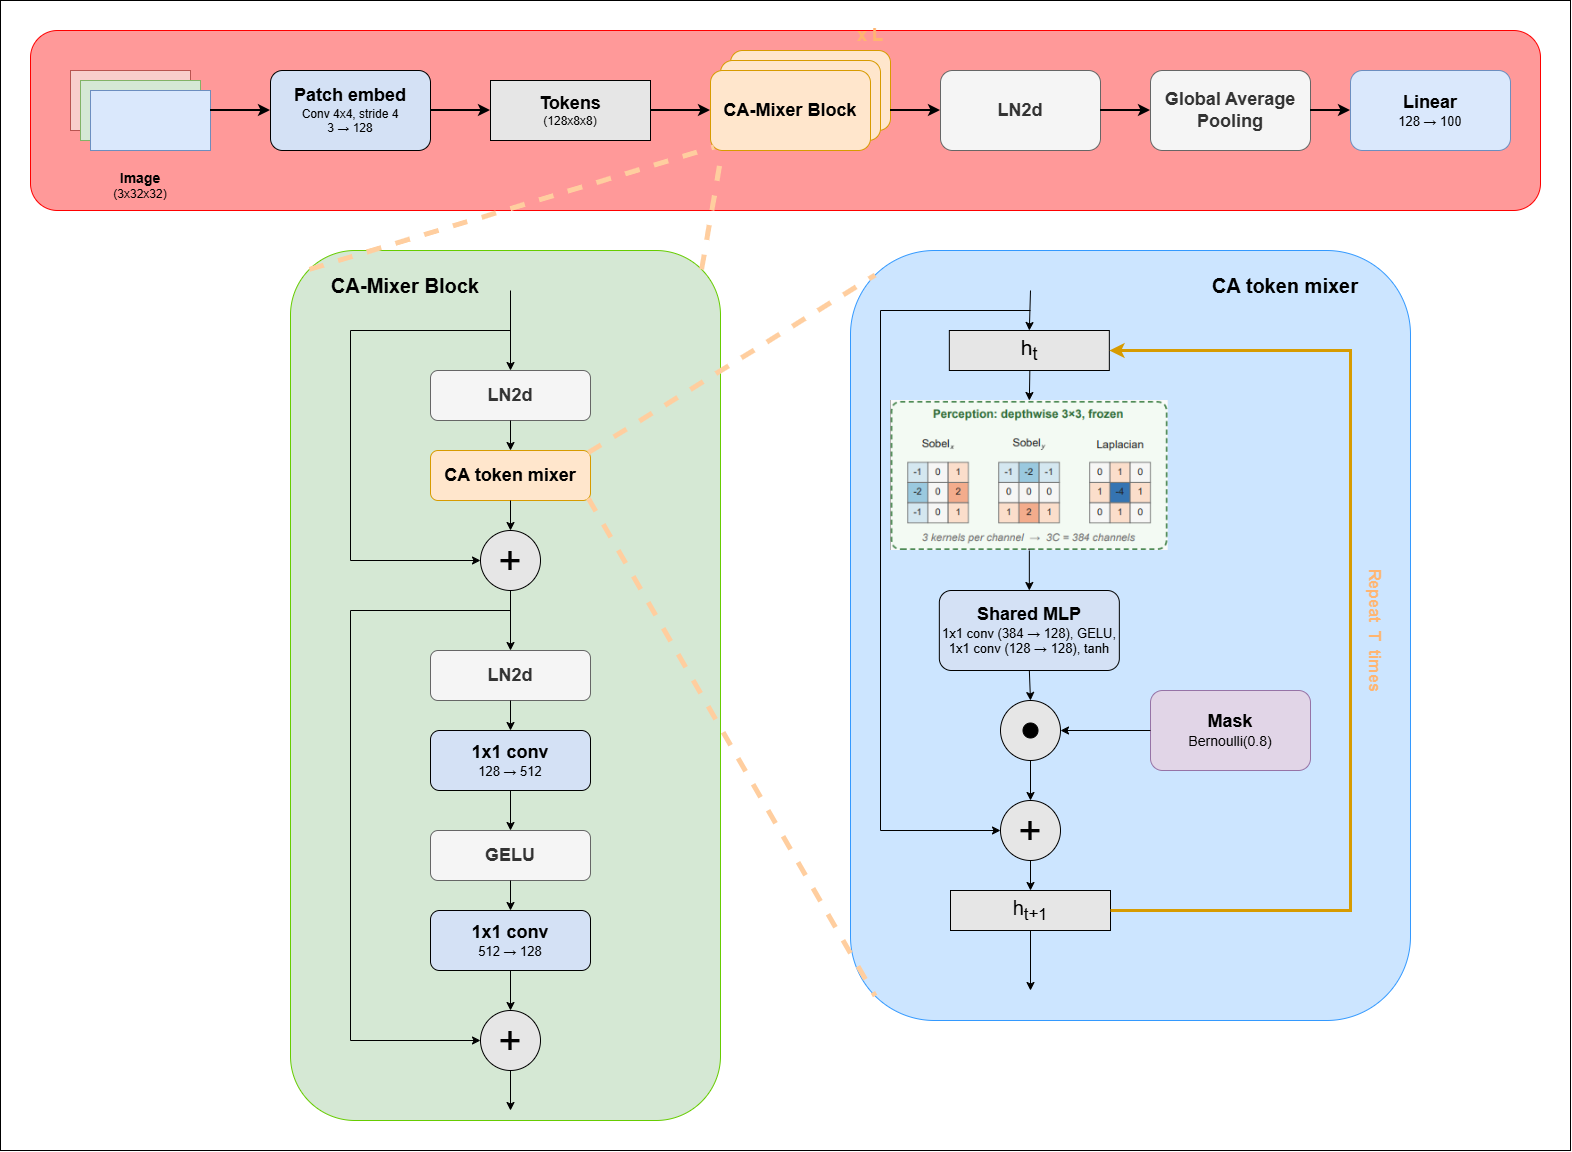
\includegraphics[width=0.92\textwidth]{figures/ca-mixer_model_architecture.png}
\caption{Macro-architecture and block design of CA-Mixer: patch embedding ($128 \times 8 \times 8$ tokens), CA-Mixer Block residual paths, and iterative Neural Cellular Automata (NCA) token mixer with frozen $3\times3$ depthwise Sobel/Laplacian perception kernels ($3C=384$), shared $1\times1$ conv MLP, and Bernoulli(0.8) stochastic update mask.}
\label{fig:ca_mixer_arch}
\end{figure}

\begin{figure}[htbp]
\centering
\begin{subfigure}[b]{0.92\textwidth}
    \centering
    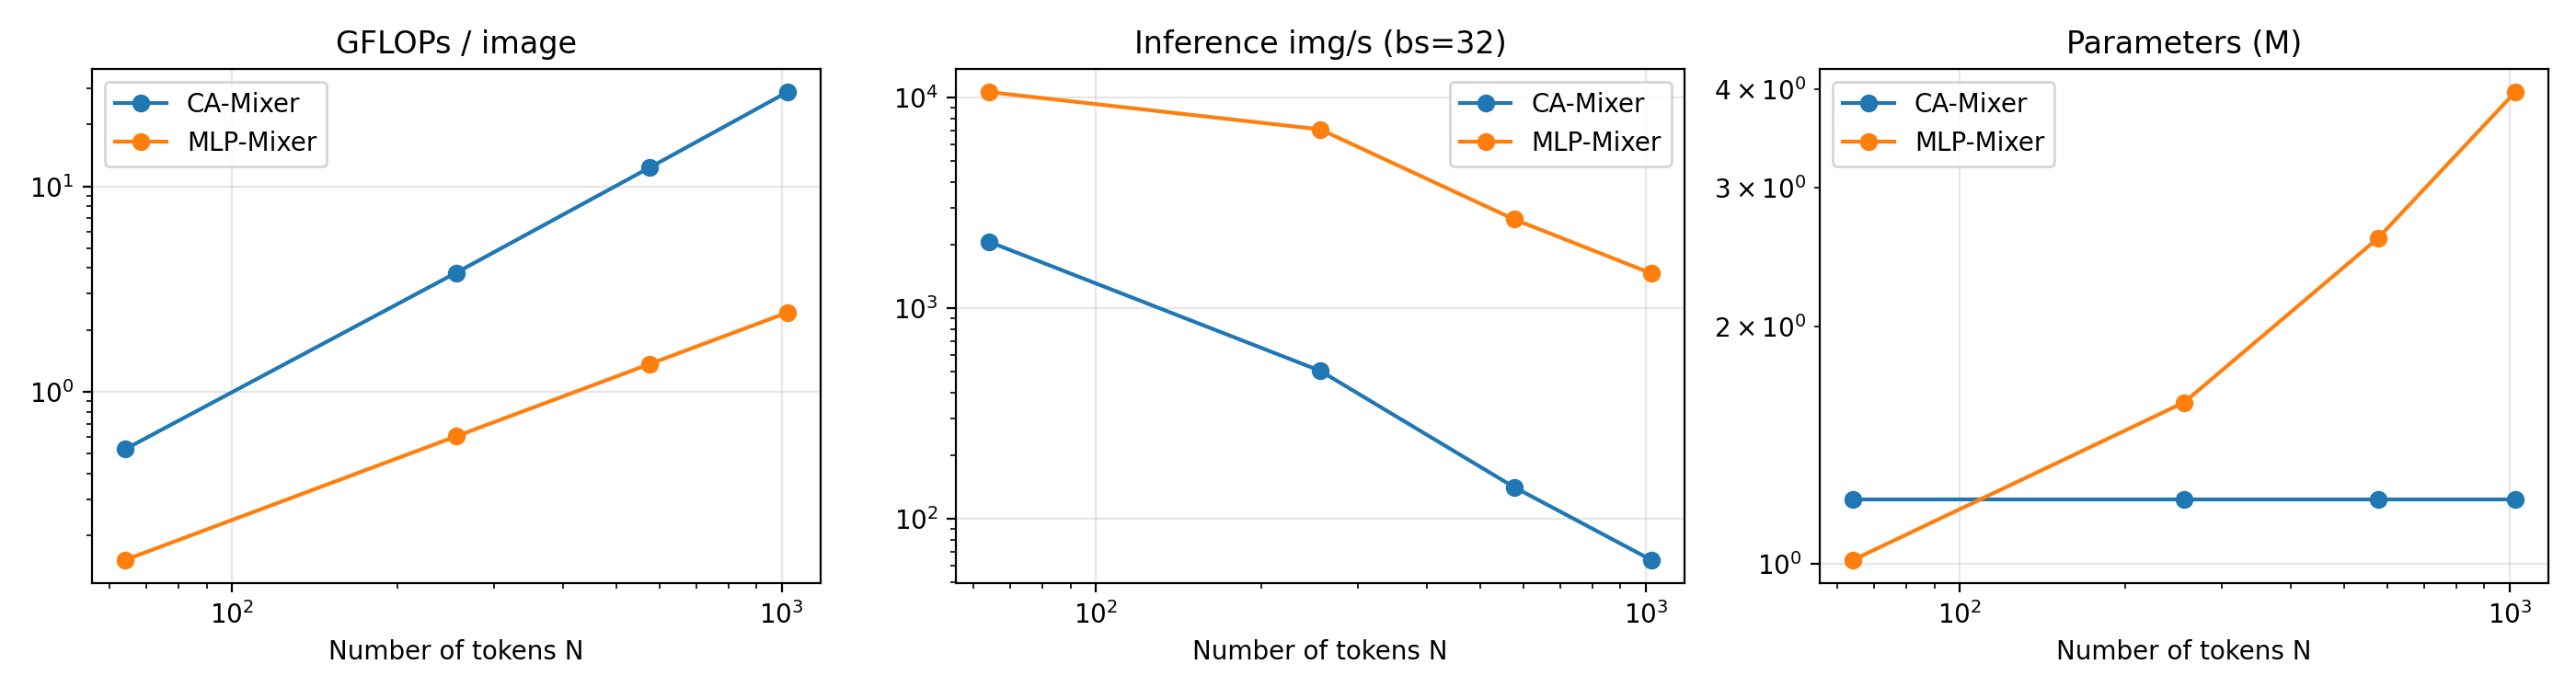
\includegraphics[width=\textwidth]{figures/fig_complexity.png}
    \caption{Parameter and FLOPs scaling vs. resolution.}
    \label{fig:ca_complexity}
\end{subfigure}
\vspace{0.5em}
\begin{subfigure}[b]{0.65\textwidth}
    \centering
    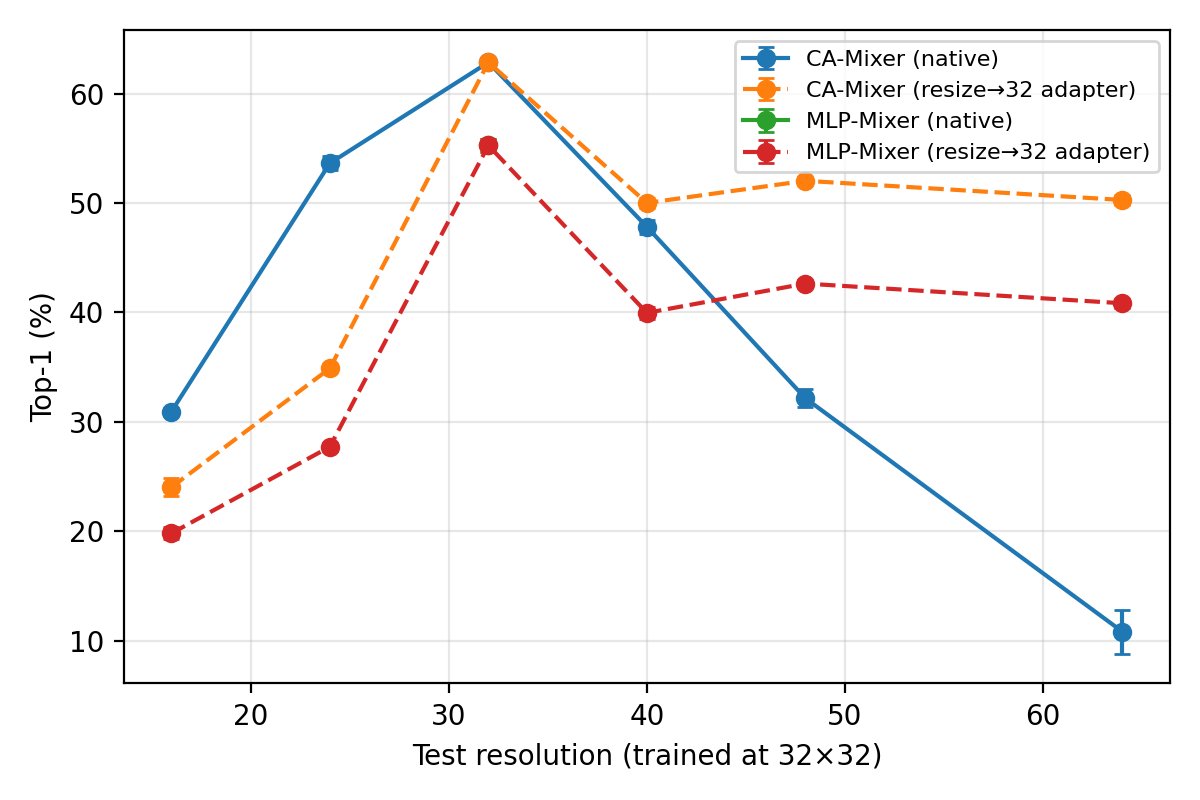
\includegraphics[width=\textwidth]{figures/fig_resolution.png}
    \caption{Zero-shot accuracy across resolutions.}
    \label{fig:ca_resolution}
\end{subfigure}
\vspace{0.3em}
\caption{Resolution invariance characteristics of CA-Mixer: constant parameter scaling and robust zero-shot accuracy under native resolution variations.}
\label{fig:ca_scaling}
\end{figure}

\textbf{Local differential perception operator} convolves the hidden state $\mathbf{h} \in \mathbb{R}^{B \times C \times H \times W}$ channel-wise with fixed, non-trainable spatial kernels $\mathbf{K} = [\text{Sobel}_X, \text{Sobel}_Y, \text{Laplacian}] \in \mathbb{R}^{3 \times 1 \times 3 \times 3}$. These biologically inspired filters capture directional spatial gradients and curvature without requiring learnable parameters.

\textbf{Shared update MLP} computes cell state increments $\mathbf{d}$ using shared $1*1$ convolutions across all spatial positions:
\begin{equation}
\mathbf{d} = \tanh\Big(\text{Conv}_{hidden \rightarrow C}\big(\text{GELU}(\text{Conv}_{3C \rightarrow hidden}(\mathbf{p}))\big)\Big),
\end{equation}
where $\mathbf{p}$ is the concatenated perception representation of dimension $3C$.

\textbf{Stochastic firing mask} introduces asynchronous update dynamics by sampling a binary mask $\mathbf{m} \sim \text{Bernoulli}(p = 0.8)$ during training. This prevents cells from over-relying on synchronous coordination and acts as strong spatial regularization.

\textbf{Iterative communication loop} repeats the state updates for $T = \max(H, W)$ recurrence steps:
\begin{equation}
\mathbf{h}_{t+1} = \mathbf{h}_t + \mathbf{m} \odot \mathbf{d}_t.
\end{equation}

\textbf{Resolution invariance property} ensures that because all perception and update operators are local 2D convolutions, the parameter count is completely decoupled from the spatial resolution $H \times W$. The compact model maintains exactly 1.21M parameters (1,207,524) while the scaled parameter-matched model maintains exactly 1.90M parameters (1,901,100) whether evaluated on $32*32$, $64*64$, or $128*128$ (Figure~\ref{fig:ca_scaling}).

\subsection{MetaFormer and Hybrid Paradigms: PoolFormer-S12 and HybridFormer}
\label{subsection:poolformer_hybridformer}

To contextualize our MLP models within the broader MetaFormer framework~\cite{yu2022metaformer}, we also analyze two hierarchical architectures: PoolFormer-S12 (Figure~\ref{fig:poolformer_arch}) and HybridFormer (Figure~\ref{fig:hybridformer_arch}).

\begin{figure}[htbp]
\centering
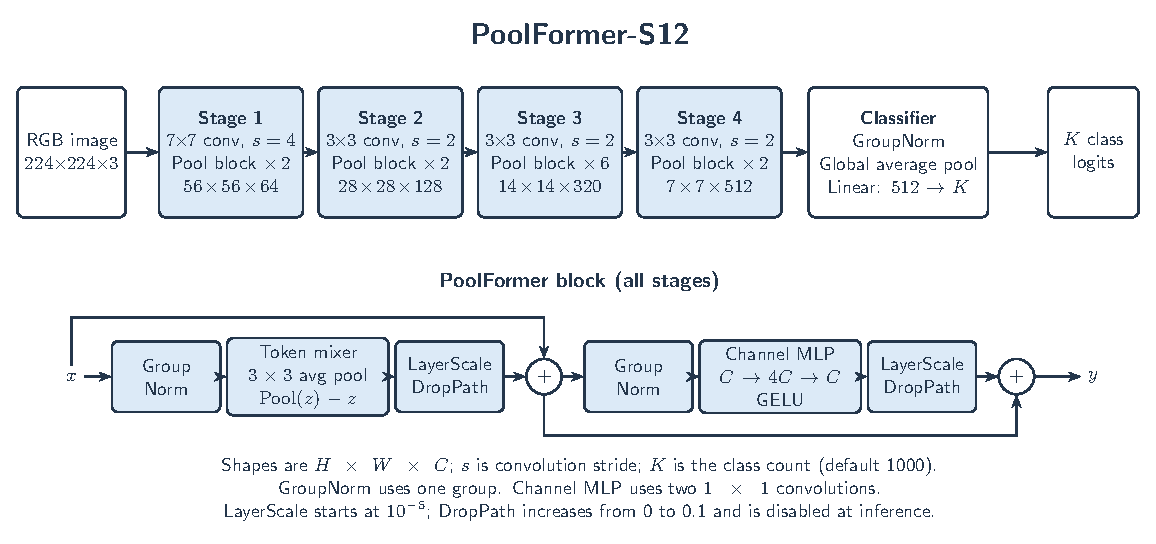
\includegraphics[width=0.98\textwidth]{figures/poolformer_arch.pdf}
\caption{Macro-architecture and block design of PoolFormer-S12: 4-stage hierarchical downsampling using non-parametric $3\times3$ average pooling for spatial token mixing.}
\label{fig:poolformer_arch}
\end{figure}

\begin{figure}[htbp]
\centering
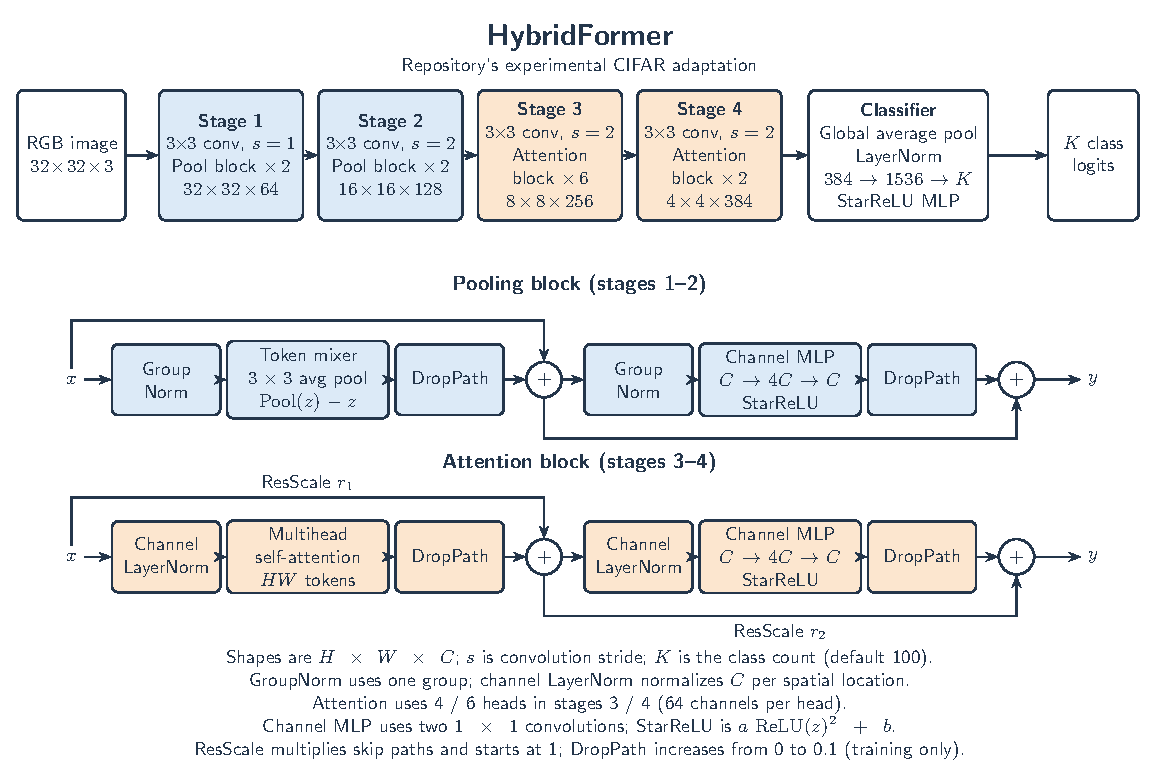
\includegraphics[width=0.98\textwidth]{figures/hybridformer_arch.pdf}
\caption{Macro-architecture of HybridFormer on CIFAR-100: combining parameter-free pooling blocks in Stages 1--2 with Multi-Head Self-Attention blocks in Stages 3--4 alongside StarReLU channel MLPs.}
\label{fig:hybridformer_arch}
\end{figure}

\subsubsection{PoolFormer-S12 Architecture}
\label{subsubsection:poolformer}

PoolFormer-S12 verifies the foundational premise of MetaFormer: that the macro-architecture itself, rather than specific token mixer parameters, delivers strong visual representations~\cite{yu2022metaformer}.

\textbf{Four-stage hierarchical downsampling} organizes the network into four stages with depths $[2, 2, 6, 2]$ and channel dimensions $[64, 128, 320, 512]$ (Figure~\ref{fig:poolformer_arch}). On $224*224$ inputs, a $7*7$ patch convolution stem with stride 4 reduces spatial resolution to $56*56$, followed by $3*3$ stride-2 convolutional downsamplers between subsequent stages.

\textbf{Non-parametric average pooling token mixer} replaces self-attention with a parameter-free spatial pooling operation:
\begin{equation}
\text{TokenMix}(\mathbf{x}) = \text{AvgPool2d}(\mathbf{x}, k=3, s=1, p=1) - \mathbf{x}.
\end{equation}
Subtracting the input tensor computes a residual difference representation without introducing a single learnable spatial weight.

\textbf{Channel MLP and normalization} refine features via two $1*1$ convolutions with expansion ratio 4 and GELU non-linearity, combined with GroupNorm (1 group, equivalent to LayerNorm over channels) and LayerScale initialized to $10^{-5}$. The complete architecture contains 11,453,476 parameters.

\subsubsection{HybridFormer Architecture}
\label{subsubsection:hybridformer}

HybridFormer combines parameter-free pooling with Multi-Head Self-Attention (MHSA) across hierarchical stages (Figure~\ref{fig:hybridformer_arch}).

\textbf{Multi-stage hybrid token mixing} assigns distinct mixing mechanisms to different resolution regimes: lightweight parameter-free pooling blocks in high-resolution early stages (Stages 1 and 2, at $32*32$ and $16*16$), and Multi-Head Self-Attention in low-resolution late stages (Stages 3 and 4, at $8*8$ and $4*4$). This avoids the quadratic complexity of self-attention on large token grids while preserving long-range relational reasoning in deep semantic stages.

\textbf{Multi-head self-attention with ResScale} in Stages 3 and 4 processes $HW$ tokens using 4 heads (Stage 3) and 6 heads (Stage 4) with head dimension 64, paired with channel LayerNorm and learnable skip scaling ($r_1, r_2$).

\textbf{StarReLU channel MLP} equips the feedforward network with StarReLU activation:
\begin{equation}
\text{StarReLU}(x) = s * (\text{ReLU}(x))^2 + b,
\end{equation}
where $s$ and $b$ are learnable scale and bias parameters. On native $32*32$ CIFAR-100 images, HybridFormer comprises 10,594,622 parameters.
